The purpose of this introduction is to set the stage for the rest of
this dissertation part and the research presented herein. Here I will
establish the merit and relevance of the presented work. The problems
approached here apply to a variety of active areas of study and modern
applications within the fields of acoustics and fluids, though the
primary focus and motivation of this work, is better understand the
physics related to specific biological effects of
\ac{DUS}. Accordingly, I describe the driving physical mechanisms of
interest to these problems, which are studied. The framework from
which I approach these problems by modeling tissue as a compressible
fluid system is also discussed. Finally, an overview of the goals and
contributions of this thesis are presented.

\section{A physical description of sound}
Sounds are molecular-scale vibrations traveling through a
medium. Atoms and molecules perturbed or displaced collide with
neighboring atoms and molecules, which collide with their neighbors
and so on. In this way, mechanical energy propagates as a wave, away
from the initial perturbation location, through any gas, liquid, or
solid medium. This is the basic mechanism by which sound moves through
all matter whether it be the tissues in human body, the water in the
oceans, or the plasma in the stars. Through years of study and
experimentation, man has gained a deep understanding for the physical
behavior of sound and has learned to harness it as a tool, leading to
high-impact advancements throughout \ac{STEM} in areas ranging from
climate change to structural health monitoring and diagnostic and
therapeutic medicine. While much of our basic understanding of sound
has come from the theoretical study of sound propagating through a
constant, infinite, homogeneous medium, there is no such medium in
reality, and many of the interesting physical questions and real
world applications of sound are concerned with the scenarios in which
sound acts to physically alter the medium through which it is
traveling.

The focus of this part of thesis is on problems in which sound travels
between multiple media in such a way that the media themselves are
physically changed or affected. Typically, when sound traveling in one
medium encounters another medium, a portion of the acoustic energy is
transmitted into the new medium, while the remainder is reflected
and scattered back into medium from which the sound originated. In
most cases, this results in little change in the media themselves,
however, in some instances, acoustic energy can be converted into
other forms of energy such as kinetic or thermal, resulting in bulk
motion or heating of the media respectively. An example of this is a
gas-vapor bubble within water or tissue driven by an acoustic wave. As a result
of rising and falling acoustic pressure the bubble may oscillate or
collapse, changing the temperature or pressure within the bubble and
driving the motion of the surrounding medium. Another example is the
dissipation of acoustic energy as heat through viscous mechanisms,
resulting in a temperature rise in a viscous medium with an acoustic
field. The resulting thermal or physical stresses associated with the
heating or movement of the media may result in a physical change (eg.,
phase change) or chemical change (eg., denaturation of proteins in
tissue). The ability of acoustic waves to physically alter a media is
of particular interest to the field of medical ultrasound, in which it
is relevant to both safety concerns in the context of diagnostic
sonography and engineering concerns in the context of therapeutic
\ac{US}.

\section{Ultrasound in medicine and biological effects}
The use of ultrasound in medicine dates back to the 1940s, when
Austrian neurologist Dr. Karl Theodore Dussik attempted to use
transmission ultrasound to outline the ventricles of the brain
\citep{Dussik1942,Singh2007}. Since then the abilities and use of
\ac{US} have expanded greatly and the technology has proven to be a
powerful tool for noninvasive therapies and safe, real-time diagnostic
imaging. Consequently, the use of \ac{US} has become ubiquitous
throughout modern medicine.

For context, I will explain the basic physical processes that occur
during \ac{US} procedures. In practice, high-frequency, typically MHz
range, acoustic waves and pulses are created at the surface of the
body using a piezoelectric \ac{US} transducer. These vibrations, or
acoustic waves, propagate via an impedance matching, acoustic coupling
medium from the transducer into the tissue. Once in the tissue, a
portion sound scatters at material interfaces within the body, where
acoustic impedance changes, or more simply, some of the sound echoes
whenever it moves from one tissue to another, or encounters a cavity
in the body. This scattering of sound is the basic physical principle
that makes the use of ultrasound for diagnostic imaging possible. In
\ac{DUS}, scattered echoes are picked up by a receiver, recorded, and
processed. The strength and timing of these echoes are used to
generate a real-time image of the scattering surface. This passage of
acoustic waves through tissue does not typically directly alter or
affect the tissues structures or processes and the use of ultrasound
for imaging is typically considered safe and noninvasive. Despite
this, this process is not entirely passive. When energy from
ultrasound is converted to kinetic or thermal energy, within tissue,
it can physically alter or damage that tissue through a variety of
mechanisms. These effects to the body are referred to as \ac{US}
bioeffects. In therapeutic applications, \ac{US} is used to
intentionally cause desirable bioeffects that are beneficial to the
patient. In the case of diagnostic ultrasound, bioeffects are
generally undesirable side effects that are avoided if
possible. Ultrasound bioeffects have motivated extensive research for
use in the development of effective guidelines and regulations for the
development and use of safe \ac{US} technologies and
procedures. 

A large portion of past research into ultrasound bioeffects has
focused on determining what types of \ac{US} bioeffects exist, and
under what circumstances they occur. This work has shown that
bioeffects may take on a variety of different forms, depending on the
\ac{US} parameters and type of tissue exposed. Various kinds of
hemorrhage and cell death are among the most common forms of \ac{US}
bioeffects. In gaseous tissues such the lung and intestines,
ultrasonically induced hemorrhage has been
observed. \cite{Lehmann1953} and \cite{Miller1994} observed abdominal
petechial hemorrhage as a result of unfocused ultrasound in mice. And
\cite{Child1990} found hemorrhage in mouse lungs after the animal was
exposed to lithotripter pulses. Numerous other studies have been
performed on the topic of US-induced lung hemorrhage and a much deeper
review can be found in chapters \ref{ch:usbe_lung} and
\ref{ch:usbe_lung_bio}. Pulsed ultrasound of the heart has been shown
to be capable of inducing cardiac contractions in frogs and mice
\citep{Dalecki1993,MacRobbie1997}. Cell death has been observed in
liver, kidney, and heart as a result of \ac{CEUS}, which uses
injections of contrast microbubbles as additional scattering surfaces
\cite{Skyba1998, Miller2008a}. In this thesis I will use computational
models to investigate bioeffects resulting from \ac{CEUS} and
\ac{DUS}-induced lung hemorrhage.

\section{Tissue as a compressible fluid system}
To investigate \ac{CEUS} and \ac{DUS}-induced lung hemorrhage,
throughout this dissertation I will be modeling the relevant physical
problems of ultrasound in human tissue as compressible, multiphase
fluid systems. In this section I will attempt justify this general
approach and explain some of the applicable assumptions and
implications.

The underlying governing equations upon which each of our models are
based are the general conservation equations for mass, momentum, and
energy for a fluid,
\begin{subequations} \label{eq:intro_conservation}             
  \begin{align}
    \frac{\partial \rho}{\partial t} + \nabla\cdot\left(\rho\bs{u}\right) =& 0,\\%
    \rho\frac{D \bs{u}}{D t} =& \nabla\cdot\bs{\tau}+\bs{g},\\%
    \frac{\partial E}{\partial t} + \nabla\cdot\left(E \bs{u}\right) =& \rho\left(\bs{g}\cdot\bs{u}\right) + \nabla\cdot\left(\bs{\tau u}\right) + \nabla\cdot\bs{q},%
  \end{align}
\end{subequations}
where $\rho$ is density, $\bs{u}$ is the flow velocity vector, $t$ is
time, $\bs{\tau}$ is the stress tensor, which is a second order
tensor. $\bs{g}$ is the body force vector,
$E = \rho \left(e + \frac{1}{2}\left[\bs{u}\cdot\bs{u}\right]\right)$
is the total energy defined as the sum of the kinetic energy per unit
mass $\frac{1}{2}\left(\bs{u}\cdot\bs{u}\right)$ and the internal
energy per unit mass $e$, and lastly $\bs{q}$ is the heat flux
vector. To model ultrasound-tissue interactions, the general
conservation equations \eqref{eq:intro_conservation} are simplified
and manipulated based on the physics appropriate to the specific
problem at hand. The closure of these equations is also treated
differently depending on the particular problem and model. Details on
the appropriate equations of state used to relate pressure and energy,
constitutive equations used to relate stress and strain, and boundary
conditions are described in greater detail in sections
\ref{subsec:usbe_bubble_model} and \ref{subsec:governing_equations}.

To consider what physical effects are at play during diagnostic
ultrasound, both contrast-enhanced and of the lung, I consider the
basic physical scenario of each of these problems. That is an acoustic
wave travels through a multiphase medium consisting of soft tissue and
gas. Soft tissues are viscoelastic materials, i.e., they exhibiting
solid and fluid like behaviors, i.e, viscous and elastic effects may
be simultaneously at play. These tissues include blood as well as
lung, liver, and kidney tissue, which are relevant to the motivations
of this thesis. The multiphase component of these problems suggests
that gas-liquid/gas-viscoelastic interface phenomena such as surface
tension may also be of some relevance. As fluid motion is expected,
inertial effects will likely be of importance. Additionally, as
ultrasonic heating is a known source of biological effects, I consider
this possibility as well. And for completeness, since the vast
majority of ultrasound procedures do not occur on the International
Space Station, I consider the effects of gravity too. In the following
two sessions, I introduce dimensional analysis to assess the relative
importance of each of these physical phenomena for the problems we
approach in this part of the thesis.

\subsection{Dimensional analysis and assumptions for Contrast Enhanced Ultrasound}
\ac{CEUS}-related bioeffects are generally attributed to a process
called \ac{IC} in which a bubble or void within a fluid collapses
rapidly. This can result in high temperatures, pressures, stresses,
strains, and strain rates within the surrounding fluid. More details
about this process and its relationship to \ac{US} bioeffects will be
provided in Section \ref{subsec:bioeffects_mechanisms_ceus}. In this
work, I consider the problem of a single \ac{US} pulse impinging upon
a contrast agent microbubble, initially at rest within a viscoelastic
soft tissue. For the sake of justification I consider a typical
case here. In Chapter \ref{ch:usbe_bubble} a more in-depth
analysis, specific to the work presented, is performed. Consider an
ultrasound pulse of clinically relevant frequency $f = 3$ MHz and
\ac{PRPA}$=p_a = 1$ MPa. The soft tissue is treated as a Voigt
type viscoelastic material as in \citep{Yang2005} and has a nominal
density of $\rho = 1000$ kg/m$^3$, an elastic modulus ranging from $G = 10$ kPa to $1$
MPa, and a viscosity of $\mu = 0.015$ Pa s. Surface tension will be
based on water such that $S = 0.056$ N/m. Consider a
characteristic velocity of $u = \sqrt{p_a/\rho} = 31.6$ m/s. Note
that the physical properties of soft tissue vary widely and are poorly
characterized, particularly at the strain rates associated with
cavitation. As a characteristic length scale, I use a typical
bubble size such that equilibrium radius is $R_0 = 1\mu$m.

Based on this setup I perform dimensional analysis to assess the
relative importance of each of the potentially relevant physical
mechanisms to the problem of acoustically-driven cavitation in soft tissue:\\

\noindent\textit{Viscosity:} To access the relevance of viscosity I consider a
Reynolds Number, which is defined as $Re = \rho u R_0/\mu=2.1$ and is
a measure ratio of inertial to viscous forces in a flow. A Reynolds
number of order unity, suggests that viscous effects
are non-negligible relative to inertia and cannot be neglected.\\

\noindent\textit{Heat transfer and thermal effects:} In consideration of the
role of heat transfer, I calculate a characteristic time scale for
heat transfer $t_{thermal}=R_0^2/\alpha$, where $\alpha$ is the
thermal diffusivity, which is $\alpha = 0.143\times10^{-6}$ m$^2$/s in
water such that $t_{thermal} = 7 \mu$s. This is compared to the
approximate timescale for a spherical vapor bubble to collapse to its
minimum radius, neglecting surface tension, which is approximately
$t_{collapse} = 0.915\sqrt{\rho R_0^2 / p_a} = 29$ ns
\citep{Brennen2003}. Note that the form of the equation presented here
is for the case where the vapor pressure in the bubble $p_v$ is much
smaller than the driving pressure $p_a$, which is true for
ultrasonically driven cavitation. Here, $t_{collapse}<<t_{thermal}$, suggesting that minimal heat transfer
will occur during the collapse. This is perhaps unsurprising, as heat
transfer is generally regarded as a much slower process than
\ac{IC}. In any case, heat transfer into and out of the bubble will be
neglected in relevant analysis.\\

\textit{Surface Tension:} The Weber number is defined as
$We = \rho u^2 R_0/S = 17.9$ and represents the ratio of surface tension
to inertial forces in the flow. The calculated $We$ suggests that
surface tension at the bubble wall is not negligibly small when the
bubble is at its equilibrium radius. Additionally, I note that the
effects of surface tension may have an even greater effect during
collapse when the bubble radius may decrease by an order of magnitude
or more. Hence surface tension will not be neglected.\\

\noindent\textit{Elasticity:} The Cauchy number is defined as
$Ca = \rho u^2 / G = 1 - 100$ for the range of elastic moduli
considered (i.e., $1000$ - $5$ kPa). Based on this the effects of elasticity are not expected
to be particularly important to the bubble dynamics for the tissues of
$kPa$ order elasticity, though this is expected to change for stiffer
tissues. Accordingly, elasticity will be included
in the cavitation bubble model.\\

\noindent\textit{Gravity:} The Froude number is defined as
$Fr = u/\sqrt{g R_0}=10^4$ and is a measure of the ratio of inertial to
gravitational forces, or more generally, any applicable body
forces. The calculated Froude number suggests that gravitational and
buoyancy effects are minimal relative to inertia and will be neglected
for the sake of this analysis. This is of particular importance
because it allows us to consider the case of a radially symmetric
collapse, which greatly simplifies the problem.\\

In summary, based on the dimensional analysis performed, I will
consider axially symmetric bubble dynamics in a Voigt-Viscoelastic
medium with surface tension. The effects of gravity and heat transfer
will be neglected.

\subsection{Dimensional analysis and assumptions for acoustically driven alveolus}%
\label{sec:lung_assumptions}%
The work presented work is specifically interested in the problem of
an ultrasound pulse impinging upon an alveolus within an adult human
lung. To access the relevant physical mechanisms here in order to
layout the logic for my assumptions and approach, I present a general
case relevant to the motivating problem of lung ultrasound. A more
comprehensive justification and analysis, specific to the work
presented can be found in chapters \ref{ch:usbe_lung} and
\ref{ch:usbe_lung_bio}. Consider an ultrasound pulse with central
frequency $f = 3 MHz$, and amplitude $p_a = 1$ MPa, which are within
the expected parameter range based on past research
\citep{Miller2015a}. I will use the mean diameter of a typical adult
human alveolus as a characteristic length scale length scale
$\ell_A = 200 \mu$m \citep{Ochs2004}. The alveolus is treated as being
filled with air such that the sound speed is $c_A=343$ m/s, the
density is $\rho_A = 1.2$ kg/m$^3$, the kinematic viscosity is
$\nu_A = 16.6 \mu$ m$^2$/s, and no elasticity is present in the
alveolar interior. The surrounding soft-tissue is treated as
water-like, but with elasticity such that the sound speed is
$c_T=1500$ m/s, the density is $\rho_T=1000$ kg/m$^3$, the viscosity is
$\nu_T = 0.7 \mu$m$^2$/s and the elastic modulus is $G = 5$ kPa
\citep{Cavalcante2005}. I use a characteristic velocity
$u_a = \sqrt{p_a/\rho_A}$. Based on the physical problem described here I
use dimensional analysis to access the relative importance of
potentially relevant physical mechanisms:\\

\noindent\textit{Viscosity:} In consideration of effects of viscosity of the
dynamics of the system during the ultrasonic interface, I calculate a
viscous length scale on either side of the interface such that
$\sigma_{vA}=\sqrt{\nu_A/2\pi f}=0.94 \mu$m and
$\sigma_{vT}=\sqrt{\nu_T/2\pi f}=0.19 \mu$m. On either side of the
interface $\sigma_v << \ell$ such that the viscous layer is small
compared to the flow geometry during the ultrasonic interactions. In
recognition that the viscous layer may grow in time, after the passage
of the acoustic wave, according to $\sigma_{v}(t)\sim\sqrt{\nu t}$ we
calculate that for a $1$ kHz \ac{PRF}, the viscous layer may grow
between subsequent pulses to $\orderof{\ell}$ in the alveolar airspace
and $\orderof{0.1\ell}$ in the surrounding tissue. Hence viscosity can
be neglected for sufficiently early times, and I will do so in the
model for simplicity. I will not consider times later than
$\approx300 \mu$s to maintain reasonable accuracy of our inviscid
assumption. The applicability of this assumption in practical lung
ultrasound is aided by the fact that even higher frequencies are
sometimes used in clinical application (e.g., typical frequencies may be $f = 5$ MHz in adults and $12$ MHz in newborns) \cite{Lichtenstein2009}.\\

\noindent\textit{Heat transfer and thermal effects:} I use similar arguments to
those used for viscous effects in consideration of thermal
effects. The thermal length scale is defined as
$\sigma_\kappa=\sqrt{\kappa/\pi f \rho C_p}$, where the $C_p$ is the
specific heat and $\kappa$ is the thermal conductivity. In air
$C_{pA}=1005$ J/Kg K and $\kappa_A=0.027$ W/m K and in Water
$C_{pT}=1005$ J/Kg K and $\kappa_T=0.49$ W/m K. Hence
$\sigma_{\kappa A} = 0.3 \mu$m and $\sigma_{\kappa T} = 1.5 \mu$m. On
either side of the interface, $\sigma_\kappa << \ell$ such that the
thermal boundary layer is small relative to the characteristic length
of the flow. Hence I will neglect heat transfer in my approach to this
problem moving forward.\\

\noindent\textit{Surface Tension:} The role of surface tension in the alveoli
is critical to healthy respiratory function. Alveoli secrete pulmonary
surfactant, which lowers the surface tension at the alveolar surface,
helping prevent airway collapse and easing the re-inflation of alveoli
during breathing. As a result of this surfactant, alveolar surface
tension is far below that of water and has been reported as $S_A = 9$
mN/m \citep{Schurch1976}. Hence I define an acoustic Weber number as
$We = p_a\ell/S_A = 22222$. This suggests that forces due to surface
tension are small relative to the acoustic pressure at the
interface. Based on this, I will neglect surface tension in my
analysis as well.\\

\noindent\textit{Elasticity:} To assess the expected impact of elasticity on
the system I define an acoustic Cauchy number $Ca = \rho_T u_a^2/G$
which becomes the ratio of the acoustic pressure to the elasticity
$p_a/G = 200$. This suggests that the effects of elastic effects will
be dominated by the acoustic pressure during the wave-interface
interaction within the tissue. Within the alveolar air space, there is
no elasticity and the Cauchy number is infinite. Based on this, I will
neglect elasticity in my model. Additional calculations considering the relevance of this assumption at later times, after the passage of the wave will be provided in Chapter \ref{ch:usbe_lung_bio}.\\

\noindent\textit{Gravity:} The importance of gravity is assessed based on a
Froude number calculation
$Fr= u_a / \sqrt{g \ell} =\sqrt{ p_a/ \rho g \ell} = 714$. This
suggests that gravitational forces are small relative to inertia, and
will be neglected. Another reasonable justification for neglecting
gravity is that the orientation of the model problem in space is
arbitrary and as a 2D model I treat the flow as existing in a plane
that is orthogonal to gravitational forces and thus not unaffected by
gravity.

\subsection{Limitations} 
Before proceeding I would like to acknowledge that the simplifications
and assumptions made in the previous sections, while justified in the
specified regimes, do deviate from the true physical systems. The
purpose of these simplifications is to make the relevant problems
tractable with the available resources (computational, intellectual,
financial, temporal, etc...). There are many limitations to described
model systems that result in aspects of the true physics that are not
captured. In both \ac{CEUS} and in ultrasound-alveoli interactions,
the presented dimensional analysis is based on tissue properties such
as viscosity and elasticity and behavior that are poorly characterized
in both nature and quantity. Additionally the analysis performed here
is for reference cases within the relevant range, and certain
dependencies, such as the frequency dependence of sound speed in bulk
lung tissue, are not captured here. Furthermore, actual tissues are
highly heterogeneous and may be characterized by a wide range of
physical length scales. Despite these limitations, the purpose of this
work is to gain insight into the approximate physics applicable to
these problems, which hopefully this approach achieves.


\section{Physical mechanisms of ultrasound bioeffects} \label{sec:bioeffects_mechanisms}%
%
Depending on the type of physical damage mechanism responsible,
\ac{US} bioeffects are classified into two groups, thermal and
non-thermal. The first group, thermal bioeffects are characterized by
deposition of acoustic energy into tissue as heat and are often a
result of therapeutic, rather than diagnostic, ultrasound. This
heating can lead to a variety of deleterious effects including the
release of highly reactive free radicals and protein denaturation at
the molecular level and protein denaturation and death at the cellular
level, ultimately causing tissue damage or death. As an example, one
class of therapeutic \ac{US}, know as \ac{HIFU} uses of strong,
concentrated acoustic fields, to intentionally convert acoustic energy
to heat through viscous dissipation. This is used to raise the
temperature of unwanted tissues such as fat or cancer to destroy
it. Little else will be said about thermal bioeffects, as the
bioeffects problems of interest to this work fall into the non-thermal
category. Non-thermal bioeffects are attributed to a variety of
physical phenomena including acoustic radiation force, radiation
torque, and acoustic streaming though the bulk of non-thermal
bioeffects are commonly associated with acoustical cavitation, which
is the most widely studied non-thermal mechanisms
\citep{Dalecki2004}. For certain bioeffects, such as \ac{DUS}-induced
lung hemorrhage, the physical mechanisms is largely unknown.

The bioeffects that are of motivation and interest to this thesis are
those that can result from \ac{DUS}, which are unintentional
and a represent a potential safety concern. \ac{DUS} bioeffects tend
to be a result of mechanical processes and typically take the form of
hemorrhage, tissue damage or cell death. 

\subsection{Cavitation of ultrasound contrast agent
  microbubbles} \label{subsec:bioeffects_mechanisms_ceus}%
Acoustic cavitation is the phenomenon by which gas nano and
microbubbles, called cavitation nuclei, are cyclically grown by low
pressures within the \ac{US} field and collapsed high pressures within
the field. When the bubble dynamics during collapse are dominated by
the inertia of the surrounding fluid, it is called Inertial Cavitation
\ac{IC}. \ac{IC} is typically violent and results in the bubble
collapsing to a fraction of its original size. There are several
possible damage mechanisms associated with \ac{IC} that may be
responsible for observed \ac{US} bioeffects. Upon collapse, the
pressure and temperature within the bubbles spike, often reaching
billions of pascals and thousands of Kelvin respectively. Due to the
pressure difference between the vapor/gas mixture within the bubble at
collapse and the surrounding media, the collapsed bubble can emit a
powerful shock wave which can be damaging to the bubbles
surroundings. When cavitation is triggered near a rigid surface, the
bubble can collapse in a radially asymmetric fashion causing a high
speed ``re-entrant'' jet of liquid to impinge upon the surface,
effectively striking the surface with a liquid hammer. If cavitation
occurs at an appropriate distance from a non-rigid surface, such as
soft tissue boundaries and blood vessel walls, the jet can impinge
away from the surface, potentially invaginating the surface
\citep{Brujan2011}. Figure \ref{fig:intro_cavitation_schematic}
schematically illustrates potential cavitation damage mechanisms
within a blood vessel.
\begin{figure}
  \centering
  \def\svgwidth{0.9\textwidth}
  \import{./figs/intro_figs/}{Cavitation_schematic.pdf_tex} \hfill%
    \caption{A schematic illustration of ultrasound induced cavitation
    and potential bioeffects damage mechanisms (from top to bottom):
    a). Bubble expansion beyond the radius of a surrounding blood
    vessel. b.) A cavitation jet away from the wall of a surrounding
    blood vessel or tissue surface causes the surface to
    invaginate. c.) A cavitation jet of high speed liquid strikes a
    vessel or tissue wall. d.) A shock wave created by the bubble
    collapse encounters nearby tissue.}
  \label{fig:intro_cavitation_schematic}
\end{figure}

As a result of the potential for cavitation-related \ac{US} bioeffects
the United States Food and Drug Administration called for a metric to
predict likely cavitation damage from ultrasound. As bioeffects are
typically attributed to \ac{IC}, efforts to predict cavitation damage
considered the likelihood of \ac{IC} based on theoretical calculations
of free gas bubbles in water. In the case of acoustic cavitation, this
depends on the duration of peak negative pressure experienced by a
cavitation nucleus, with longer interactions depositing more energy
into the nucleus, and thus having a greater likelihood inducing
\ac{IC}. The duration of the \ac{PRPA} is inversely related to the
\ac{US} frequency. \cite{Holland1989} demonstrated that the threshold
\ac{PRPA} needed to trigger \ac{IC}, defined based on a maximum bubble
temperature $\geq5000$K, depended on the size of the cavitation
nucleus. Smaller cavitation nucleii, must overcome greater surface
tension effects in order to cavitate, with the Laplace pressure
scaling inversely with the radius of the nucleus. Furthermore, as
initial radius a nucleus increases, the inertia of the surrounding
fluid that must be overcome also increases\cite{AiumS72000}. Thus
\cite{Holland1989} illustrated that for a given frequency their is an
optimal nucleus size for triggering \ac{IC}. Based on these
calculations and corrections for heat dissipation in tissue the
\ac{MI} was created as a measure of ultrasound induced cavitation
related bioeffects and defined as
\begin{align}
  MI = \frac{P_{r.3}}{\sqrt{f_c}},
\end{align}
where $P_{r.3}$ is the \ac{PRPA} derated by $0.3$ dB/MHz-cm and
$f_c$ is the center frequency \cite{Apfel1991}. The United States
\ac{FDA} mandates that $MI\leq1.9$ for diagnostic imaging, though
\ac{US} bioeffects have been observed at \ac{MI} below this in case
of \ac{DUS} of mammalian lungs.

While \ac{IC} does not typically occur during non-contrast \ac{DUS},
it is of concern during \ac{CEUS}, which uses contrast-agent
microbubbles injected into patients bloodstream to act as additional
scattering surfaces. This allows for high contrast imaging and can be
used to ultrasonically image blood flow, which is useful for
diagnosing heart valve problems, liver lesions, and more
\citep{Claudon2013,Rognin2008}. However, the use of contrast agent
microbubbles can also have potential deleterious side effects. These
microbubbles can act as cavitation nuclei and the resulting cavitation
has been associated with a variety of different forms of cellular
death and damage. The precise ultrasonic thresholds for which
cavitation and bioeffects occur have been a topic of intense study and
are not completely physically described. Furthermore, the exact
physical mechanisms through which cavitation causes bioeffects are
also not clearly understood \citep{Barnett1994}.

\subsection{Ultrasound-induced lung hemorrhage}
The second \ac{US} bioeffects topic of interest to this thesis is
\ac{DUS}-induced \ac{LH}. In the relevant literature this is also
sometimes referred to more specifically as \ac{PCH}. This phenomenon was first
discovered in mice over twenty years ago by \cite{Child1990} and
has since been shown to occur in a variety of other mammals including
rats, pigs, rabbits, and monkeys \cite{OBrien1997a, Miller2012,
  Tarantal1994a}. Research into this phenomena has been in three main
areas: (1) Determining the physical mechanism of the hemorrhage; (2)
Understanding how the occurrence and severity of the hemorrhage on the
ultrasonic properties (frequency, amplitude, waveform, etc...); and
(3) Understanding how the occurrence and severity of the hemorrhage depend on
the characteristics of ultrasound subject (species, age, anesthesia,
etc...). The work in this thesis pertains primarily to the first of these
three areas.

Despite extensive previous research into \ac{DUS}-induced \ac{LH}, the
underlying physical mechanisms are still not well
understood. Furthermore, past work has shown that common \ac{US}
bioeffects mechanisms do not explain the observed injuries. Thermal
damage mechanisms appear unlikely to be the primary source of damage
as \ac{DUS}-induced lung lesions do not appear similar to those
induced by heat \citep{Zachary2006}. Furthermore, cavitation
mechanisms do not appear to be responsible, as the severity of
\ac{DUS}-induced \ac{LH} in mice increased under raised hydrostatic
pressure \citep{OBrien2000} and was unaffected by the introduction of
\ac{US} contrast agents into subjects. Both of these results are
inconsistent with what is expected of \ac{IC}-induced bioeffects. More
recent work by \cite{Miller2016} investigating acoustical radiation
surface pressure as a potential damage mechanism found that the
pressures expected in pulsed ultrasound were likely too low to
completely explain the observed hemorrhage on their
own. \cite{Simon2012} found that atomization and fountaining occurred
at tissue-air interfaces subjected to \ac{HIFU} and suggested that
this could potentially happen at diagnostic levels as well. Similarly,
works by \cite{Tjan2007,Tjan2008} model the evolution of an inviscid,
free surface subjected to a Gaussian velocity potential and find that
this can lead to the ejection of liquid droplets. They go on to say
that \ac{DUS} of the lung may similarly lead to the ejected of
droplets capable of puncturing the air-filled sacs within the
lung. The problem of \ac{US}-lung interaction is the central
motivation of chapters \ref{ch:usbe_lung} and
\ref{ch:usbe_lung_bio}. As such, a far more in-depth literature review
will be provided in these chapters. 

\subsubsection{Driven fluid-fluid interfaces}
The physical problem underlying interactions between ultrasound waves
and the various tissue and fluid layers of the body is that of a
mechanical wave traveling in one fluid encountering a second fluid of
differing physical properties. As was previously explained, this can
result in acoustic energy being converted into motion or heat. In the
case of the bubble, the relevant manifestation of this was
cavitation. Another manifestation of this is the growth of
perturbations at fluid-fluid interfaces as a result of non-uniform
velocity gradients that occur at the driven interface. Another way of
thinking of this is in terms of baroclinic vorticity, or localized
fluid rotation, generated by the misalignment of interface density
gradients and mechanical wave pressure gradients. In this dissertation
I propose baroclinic vorticity-driven strain as a potential physical
mechanism for ultrasound induced alveolar hemorrhage. In the
remaining portion of section I discuss in greater detail the
underlying physics at play here and some of the past work that has
been done to understand it.

There has been extensive past research into the physics that underlies
interactions between mechanical waves, acceleration, and fluid-fluid
interfaces. Much of this research is motivated by applications in
fusion energy and astrophysics and accordingly has sought to
investigate regimes outside of those of acoustic
interests. \cite{Taylor1950} predicted that for an interface between
two fluids of different density, if the fluid was accelerated normal
to the interface in the heavy-to-light direction, perturbations at the
interface would grow. That is to say that a ``bubble'' of light fluid
penetrates the heavy fluid, and a ``spike'' of heavy fluid penetrates
the light fluid. This is known as the \ac{RTI}. A similar topic of
past study is the \ac{RMI}, which occurs when a perturbed fluid-fluid
interface is instantaneously accelerated by a shock, causing the
interface perturbation to grow \citep{Brouillette2002,Drake2006}. This
growth is driven by a sheet of baroclinic vorticity deposited along
the interface as a result of misalignment between the pressure
gradient across the shock and the density gradient across the
perturbed interface. This physical mechanism by which these misaligned
gradients create a torque on fluid particles and generate vorticity
can be thought of in terms of a hydrostatic balance upon a
particle. Pressure gradients result in acceleration of the flow that
is inversely proportional to density. When these two gradients are
misaligned, the result is a shearing effect on the fluid and vorticity
is generated \citep{Heifetz2015}. A graphical explanations of
baroclinic vorticity generation is shown in Figure
\ref{fig:usbe_lung_baroclinic_schematic}, which has been adapted from \citep{Heifetz2015}.
\begin{figure}
  \centering
  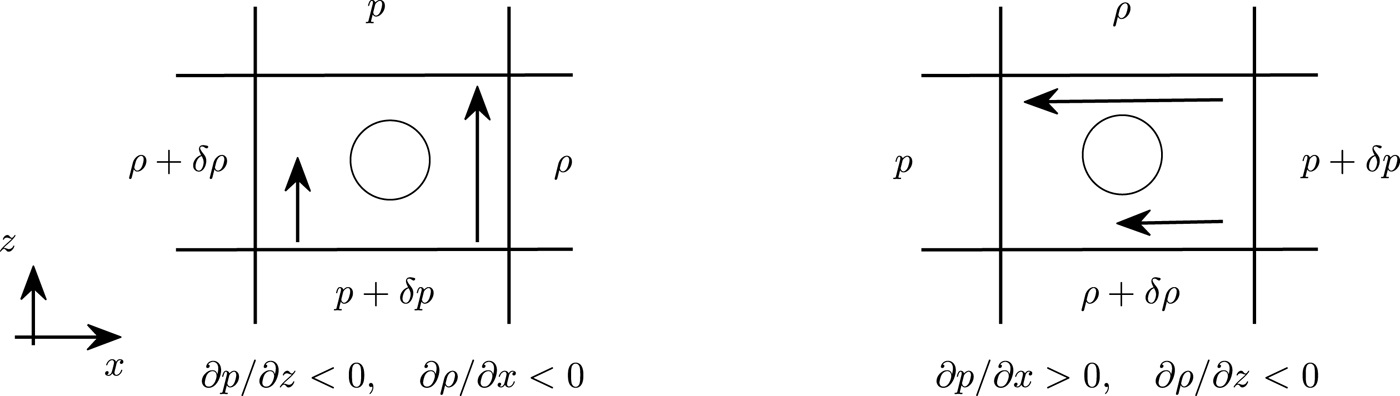
\includegraphics[width=0.9\textwidth]{./figs/intro_figs/baroclinic_schematic} \hfill
 \caption[A schematic of baroclinic torque]{From
    \cite{Heifetz2015}. A hydrostatic force balance upon a particle
    subject to perpendicular pressure and density gradients
    illustrates baroclinic torque on a fluid particle.}
  \label{fig:usbe_lung_baroclinic_schematic}
\end{figure}
Analytically, baroclinic vorticity generation can be shown by taking
the curl of the conservation of momentum equation for a compressible
fluid. It is worth noting that it is a nonlinear effect and cannot be
explained by traditional linear acoustics.

The physics of the classic \ac{RMI} are fairly well understood. For
the classical \ac{RMI} setup a planar shock impinges normally upon the
peaks and troughs of a sinusoidal interface. The interface is
accelerated non-uniformly counter-rotating vorticies are generated
across the interface. This drives peaks and troughs of the interface
to accelerate in the opposite direction. Much like in the case of the
\ac{RTI}, this too results in light fluid penetrating the
heavy fluid and vice versa. For the case of a wave moving from a light
fluid into a heavy one, the peaks and troughs of the interface
accelerate away from one another, growing the interface perturbation
perturbation. For the case of a wave moving from a heavy fluid to a
lighter fluid, the peaks and troughs interface initially accelerate
toward one another. They then pass each other, inverting the phase of
the interface perturbation, and continue moving in opposite
directions, growing the perturbation amplitude. This process is
illustrated in Figure \ref{fig:rmi_schematic}, which has been adapted
from \cite{Brouillette2002}. This work proposes that similar physics
occur at ultrasonically driven air-tissue interfaces within the lungs.
\begin{figure}
  \centering
  \def\svgwidth{0.9\textwidth}
  \import{./figs/intro_figs/}{brouillette_fig3_mod.pdf_tex} \hfill%
  \caption[A schematic view of the \acl{RMI} instability for a
  heavy-light interface]{Adapted from \cite{Brouillette2002}. The
    \ac{RMI} for a heavy-light interface is illustrated. The initial
    condition (left), circulation post wave-interface interaction
    (center), and perturbation growth (right) are shown.}
  \label{fig:rmi_schematic}
\end{figure}
 
\section{Thesis overview}
This part of the thesis presents work studying the physics of two
problems relevant to ultrasound bioeffects: 1) Cavitation of
ultrasound contrast agents microbubbles in human tissue, and 2)
\ac{DUS} of the lung. For each problem, a computational model is
developed and used to simulate the relevant dynamics in order to make
conclusions about the physics that may be relevant to the observed
biological effect.

In Chapter \ref{ch:usbe_bubble}, I simulate the cavitation bubble
dynamics of contrast agent microbubbles in soft tissue
\citep{Patterson2012}. Experimentally measured \ac{US} waves with
known bioeffects occurrence and thresholds are used
\cite{Miller2008b}.  A parametric study is performed, relating
ultrasound and tissue parameters to calculated cavitation bubble
dynamics. The soft tissue is modeled as a Voigt viscoelastic medium
based on the work of \cite{Yang2005}. The calculated cavitation
dynamics and theoretical inertial cavitation thresholds
\citep{Flynn1982,Apfel1982} are compared with bioeffects thresholds
associated with each \ac{US} pulse, as defined by the observation of
kidney hemorrhage in rats after exposure to CEUS by
\cite{Miller2008b}. While the results were generally dependent on
\ac{US}, gas, and tissue properties, it was found that the theoretical
inertial cavitation thresholds were lower than observed bioeffects
thresholds. It is shown that these thresholds correlate strongly to
calculated metrics of cavitation, such as dimensionless maximum radius
$R_{max}/R_{equilibrium}$ and that this correlation is lost when
simply looking at the dimensional maximum bubble size $R_{max}$, which
is not a cavitation metric.

In Chapter \ref{ch:usbe_lung}, I develop a model of an
ultrasonically-driven alveolus as a compressible, multi-phase fluid
system. This model is used to study the fundamental problem of an
acoustically-driven perturbed liquid-air interface. I demonstrate that
under the assumptions presented in Section \ref{sec:lung_assumptions},
strong acoustic waves of appropriate waveform are capable of
generating sufficient baroclinic vorticity to appreciably deform the
interface. The dependence of this deformation on the amplitude and
temporal characteristics of the wave is studied. It is demonstrated
that the deformation rate scales with the amount of circulation per
unit arc length of the interface. It is also shown that the amount of
circulation deposited by the wave is heavily dependent on the
deformation that occurs during the wave-interface interaction, and
therefore depends on the transient properties of the wave.

In Chapter \ref{ch:usbe_lung_bio}, the work of the previous chapter is
extended to increase its relevance to clinical \ac{US}. The model used
in the previous chapter is used to calculate the stresses and strains
induced by\ac{US} pulses on perturbed liquid-gas, similar to those of
the alveolus. These calculated stresses and strains are compared to
accepted failure criteria. It is shown that viscous stresses are small
compared to expected failure thresholds. However it is also shown that
strains at gas-liquid interfaces such as those of the lungs, driven by
acoustically-generated vorticity, may be sufficient to drive
hemorrhage for sufficiently strong ultrasound pulses. This work
concludes that while vorticity may be a possible mechanism for driving
\ac{DUS}-introduced lung hemorrhage, additional work will need to be
completed that accounts for multiple pulses as well as physical
effects of elasticity and viscosity in order fully understand the role
of vorticity in this problem.

In the final chapter \ref{ch:usbe_conclusions} of Part
\ref{part:ultrasound_bioeffects} of this dissertation, I summarize
the main conclusions takeaways and accomplishments of this work. I
Also make recommendations for future work to overcome the limitations
of the presented research and extend this work to address relevant
problems within the field.


% If the conservation  equations were kept separate
\begin{comment}
  \begin{align} \label{eq:intro_coma}
    \frac{\partial \rho}{\partial t} + \nabla\cdot\left(\rho\bs{u}\right) = 0,%
  \end{align}
  \begin{align} \label{eq:intro_como}% 
    \rho\frac{D \bs{u}}{D t} = \nabla\cdot\bs{\tau}+\bs{g},%
  \end{align}%
  \begin{align} \label{eq:intro_coe}%
    \frac{\partial}{\partial t}\left(\rho \left[e + \frac{\bs{u}\cdot\bs{u}}{2}\right]\right) + \nabla\cdot\left(\rho \left[e + \frac{\bs{u}\cdot\bs{u}}{2}\right]\bs{u}\right) = \rho\left(\bs{g}\cdot\bs{u}\right) + \nabla\cdot\left(\bs{\tau u}\right) + \nabla\cdot\bs{q}%
  \end{align}%
  \begin{align} \label{eq:stiffened_eos_intro}%
    E=\frac{\rho\left(u^2+v^2\right)}{2} + \frac{p+\gamma B}{\gamma-1}.
  \end{align}
\end{comment}


%%% Local Variables:
%%% mode: latex
%%% TeX-master: "../../main"
%%% End:
